\chapter{Introduction}
\label{chap:intro}

\section{Computer networks pervade}
Services like telephony, email and the world wide web (WWW) are a seamless part of our everyday lives. We communicate and collaborate using email, voice/video calls over Internet Protocol (IP) and online social networks. We also use web-based systems to access teaching/learning material, course registration systems on campus and even pathological examination reports. 

All of these services, and many more, are powered by several computer networks. These networks are run by commercial entities know as service providers or network operators. Examples of such network operators are: 

\begin{itemize}
\item \textbf{Cellular Network Operator:} Cellular network operators deploy and run a cellular network infrastructure. Cellular networks can also be characterized as computer networks as both the end users' devices (cell phones) and most of the devices in the infrastructure are computers. The most common services offered by these operators are voice calls and short text messages. 

A few years ago, the predominant means of connecting to the Internet was dialup over Public Switched Telephone Network (PSTN). These days, however, many end users use cellular networks to access Internet resources. In this context, the cellular network merely acts as an access mechanism to connect to an Internet Service Provider's network.


\item \textbf{Internet Service Providers (ISPs):} The Internet itself is an interconnection of ISPs networks. End users connect to the Internet by connecting to an ISP's network. This is typically done by a paid subscription to use the ISP's network. 

An ISP's network is a mostly dumb but fast carrier of IP packets, also known as IP traffic, from one point to another. The intelligence of Internet applications and the information that the Internet is so popular for, are provided by the networks run by other service providers such as the ones given below.
\item \textbf{Geo-diverse data center network operators} Today's web-based services such as Google search and Facebook have such a large subscriber base that a huge number of servers is required to run these services. To enable such services, companies like Facebook, Amazon, Microsoft and Google operate geo-diverse data centers. Servers in these data center networks run applications like Google Search, Gmail, Youtube, Twitter, Bing and Facebook.
\item \textbf{Content Distribution Network (CDN) operators:} CDNs place multiple copies of Internet resources such as web pages across the globe. The role of CDNs is to keep the latency from a user to an Internet resource small. For instance, if Google's home page were only located at a server in Mountain View, CA, the latency (the time it takes for a web browser to send a packet to the server) for users in Pakistan would be hundreds of milliseconds. Placing a replica of the Google home page close to Pakistan lowers the packet latency significantly, thereby allowing the web browser to display the page much faster.
\end{itemize}


%Shed some light on the role networks play in our lives, highlighting different types of networks.
So far, we have seen that computer networks are critical resources that enable the services that we rely on in our everyday lives. In this thesis, we will focus primarily on cellular networks and geo-diverse data centers. 

The deployment of these networks involves huge expenses. For instance, Google announced building a data center in Iowa at a cost of \$400 Million~\cite{CostOfADC}. Furthermore, according to~\cite{costcellsite}, the capital cost of a typical cellular network site is \$550,000\footnote{This does not include spectrum licensing costs. Furthermore, an operator needs to deploy many sites. A site at about every 800 meters is common in urban settings}. 

The recurring operational cost of these networks is also quite high. For instance, in 2009, Facebook spent \$50 Million on leasing the data center space, alone~\cite{FBLease}. In the context of geo-diverse data centers, other contributors to operational expenses include staff salaries, maintenance costs, the cost of inter-data center network connectivity and electricity bill. Optimizing operational costs is critical for network operators in order to offer cost-effective services to consumers and maximize their profit.

\section{Electricity costs for operational networks} 
%The significance of network electricity costs amongst various sources of operational costs in networks of different types~\cite{brill:DataCenterCrisis:UI:2007}. Let the numbers speak for themselves.
For many computer networks, electricity costs account for a significant fraction of operational costs. For instance, electricity costs may be as much as 15\% of operational costs in data centers~\cite{costCloud}. Similarly, for an operator with 7000 cellular sites in a country as small as Pakistan, the annual electricity cost can be roughly estimated at \$9.19 Million\footnote{Using a 1.5 kW draw for a single cellular site~\cite{mbakwe:btshybribpower:2011:necec}, Rs. 10 per kWh and Rs. 100 per US\$. Note that the Rs. 10 per kWh is a gross under-estimation, given that it considers only the approximate current price of the intermittently available grid power and does not factor in the cost of electricity produced using diesel generators during rolling blackouts. The cost of electricity generated through diesel generates is several times higher per kWh than the grid power.}. Telecom Italia reported a consumption of 1.793 GWh in 2012~\cite{TIAnnualReport}, which is significantly higher compared to our estimates for the Pakistani network operator and hence the electricity costs are also expected to be much higher. 

\section{The impact of energy inefficiency on operational networks' electricity costs} 
%Networks are not energy proportional and provisioned for peak workload, therefore, they are not energy efficient. This means that operators are spending way more on electricity costs than they ideally should. 

Ideally, a network's power consumption should be a linear function of workload such as the dotted line in Figure~\ref{fig:ener-prop}. The network should consume no power when there is no workload and in the presence of workload, it's power consumption should be proportional to the network's utilization. However, for most operational networks, the power consumption is well-approximated as an affine function of workload~\cite{Peng:2011:TPS:2030613.2030628,Fan:power:ICSA:2007}, as shown by the solid line in Figure~\ref{fig:ener-prop}. We say that today's networks are not energy proportional, i.e., they operate at a large fraction of their peak power consumption under no load. There are two reasons for high power consumption in the absence of workload. 
\begin{enumerate}
\item In some cases, the utilization of network hardware is nearly independent of workload. For instance, in order to allow subscribers to sense the availability of the network, it may be necessary to transmit beacon frames with no payload even when there is no traffic. Thus, the network activity under no workload conditions is not significantly less than that under peak workload. A cellular network's radio components, for instance, must continue operating and drawing power to offer uninterrupted connectivity to prospective callers, even when no call is in progress. In packet switching networks, many data link layer technologies continuously transmit frames with no payload, irrespective of traffic activity. Since the network hardware is continuously transmitting signals, it's power consumption under no load is quite high.
\item The components of the network may not be energy proportional. For instance, in data centers, server power consumption is a large fraction of the total power consumption and the server idle power consumption is a large fraction of their peak power consumption. 
\end{enumerate}

\begin{figure}
\centering
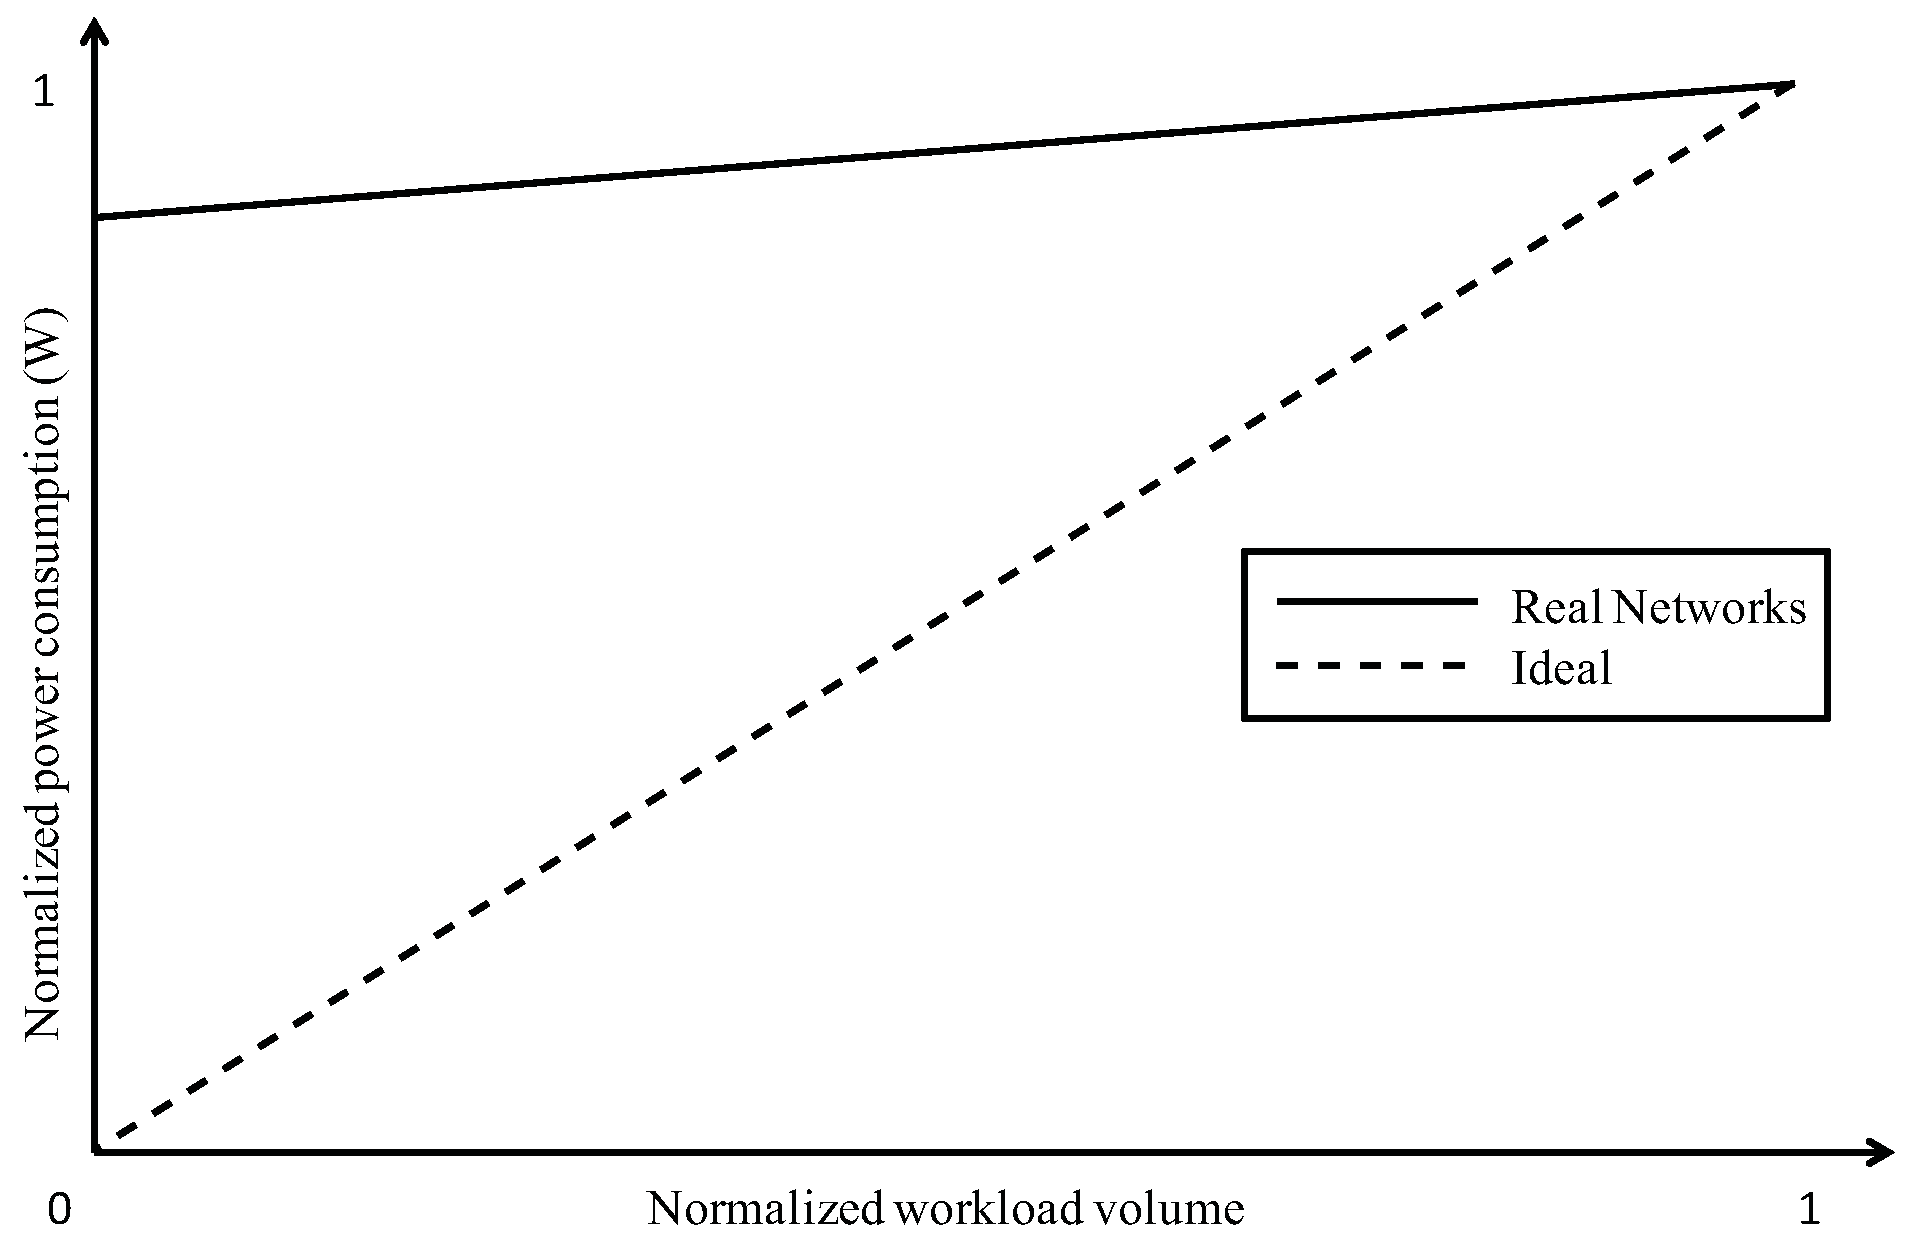
\includegraphics[width=0.7\textwidth]{pics/enerprop.eps}
\caption{Networks lack energy proportionality}
\label{fig:ener-prop}
\end{figure} 

Lack of energy proportionality is of little concern if the network consistently operates in the high workload region because in this region, the power consumption for a real network is close to ideal. However, most networks today have time-varying traffic which is in the low-workload region for considerable amount of time during a given day. Figure~\ref{fig:varwork} shows the workload for call traffic at a cellular site in a large operational GSM network in Pakistan. It shows that call traffic has diurnal cycles and that traffic peaks for only a short period of time during a day. Furthermore, the workload peak is quite high compared to the trough. ISP~\cite{1248656} and data center~\cite{10.1109/MC.2007.443} traffic also show similar trends. 

In order to meet peak expected workload amicably, networks are dimensioned according to the peak workload. Since the workload is far from the peak most of the time and networks are not energy proportional, most networks have a much higher energy consumption than what they would ideally incur. In other words, today's networks are energy inefficient. Another way to look at energy efficiency is through the lens of performance per Watt, a useful metric for energy efficiency of a network. The performance per Watt for today's networks is quite low. Therefore, it is important to lower the y-intercept of the solid line in Figure~\ref{fig:ener-prop} thereby reducing the electricity cost of today's networks without compromising on the performance that they deliver. Recent years have seen significant research focus on improving energy efficiency in both cellular and geo-diverse data center networks.

\begin{figure}
\centering
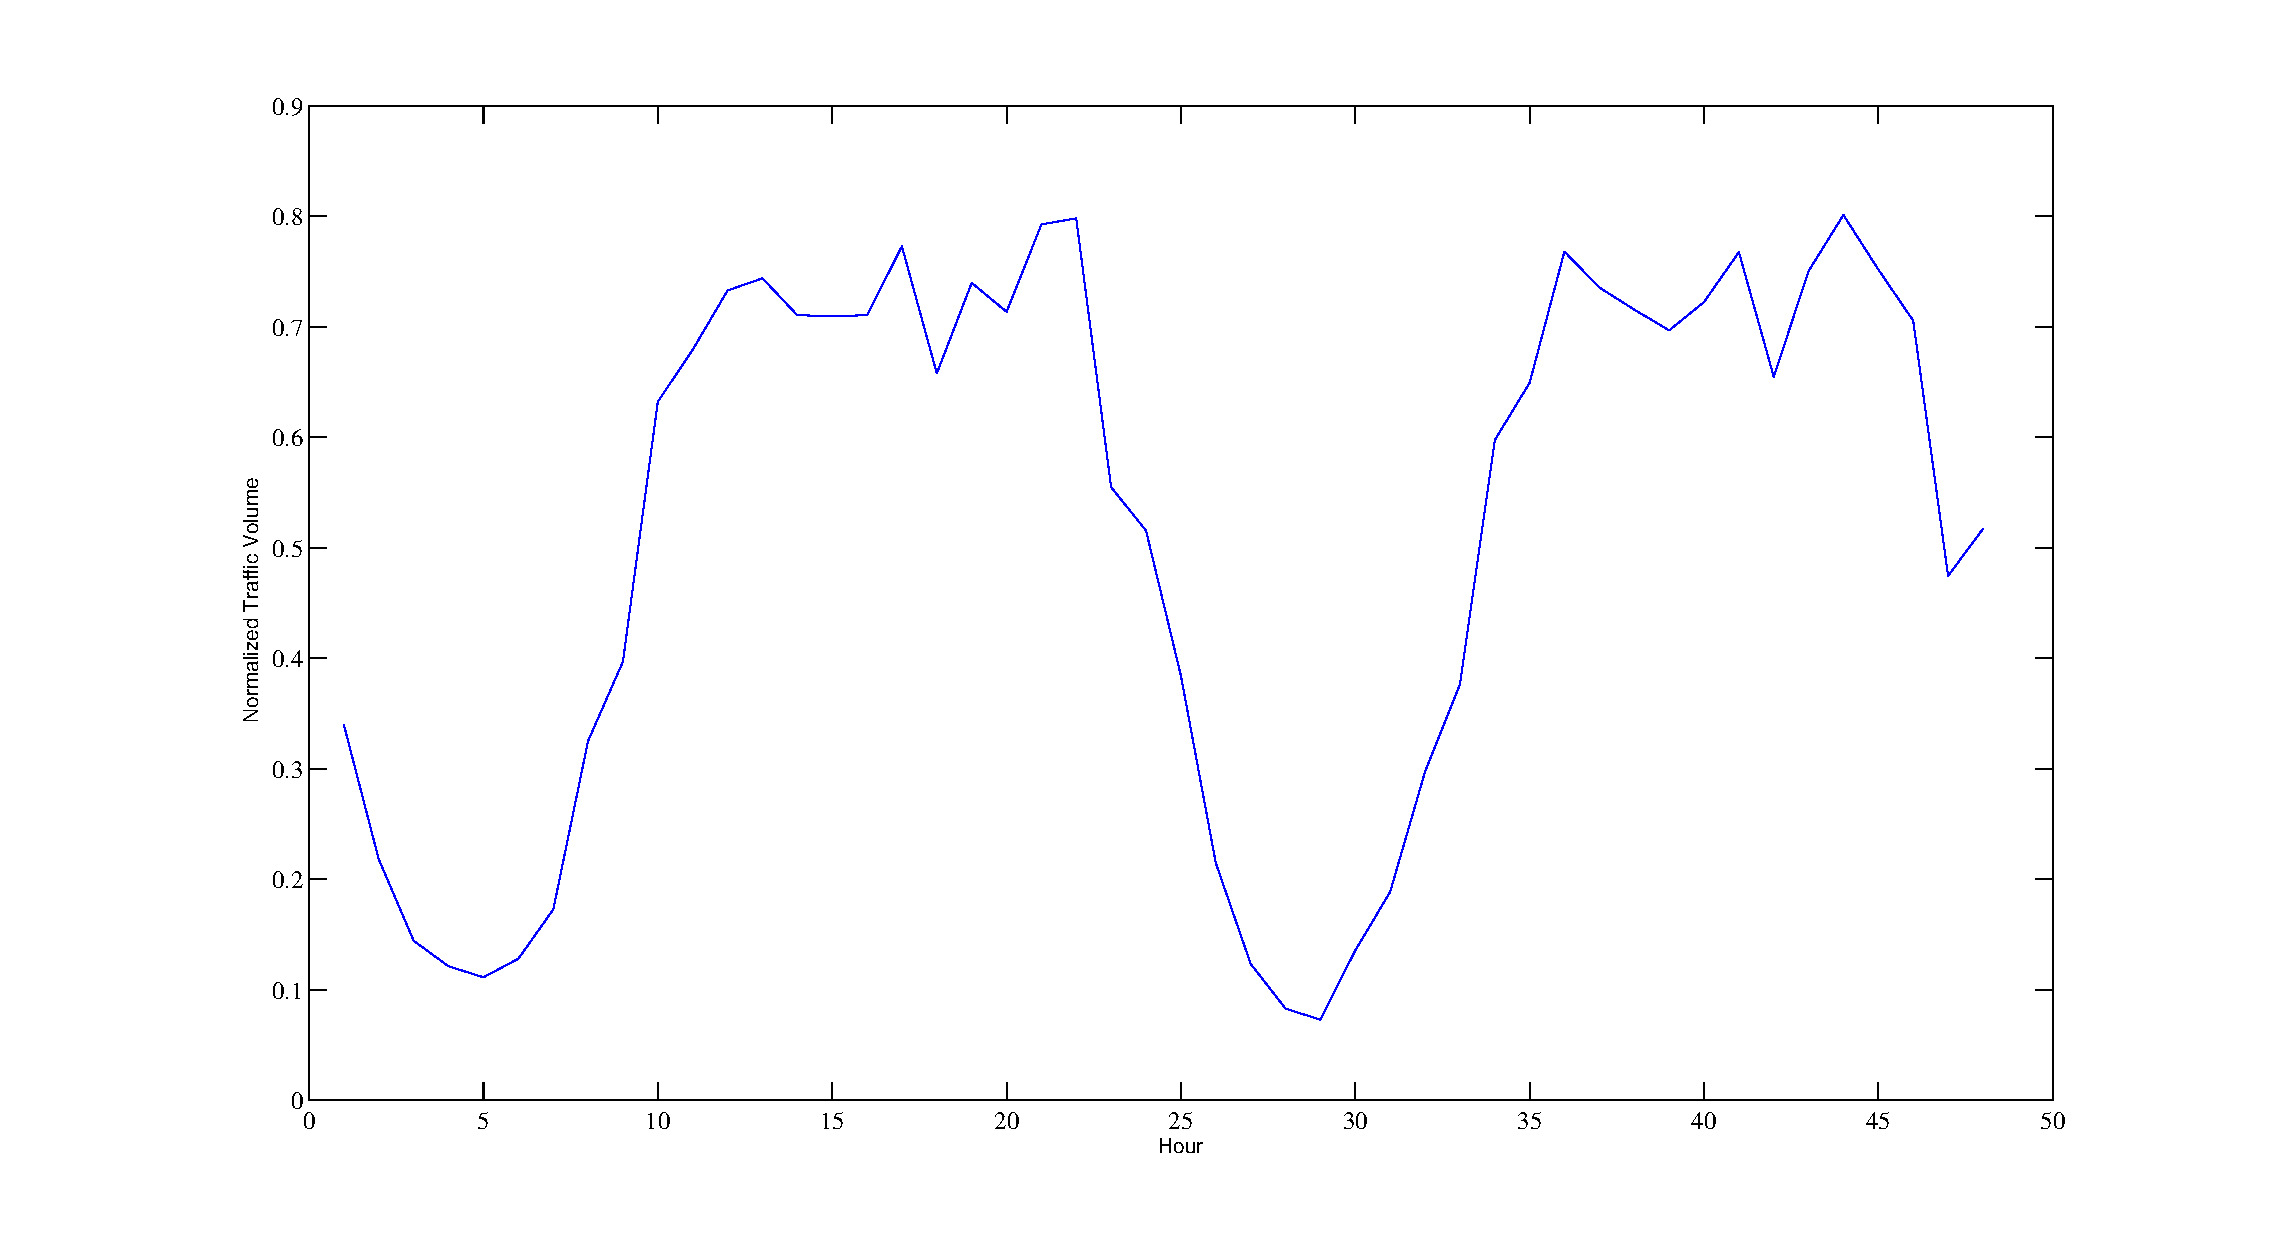
\includegraphics[width=0.7\textwidth]{pics/waridworkload.eps}
\caption{Call traffic for an oeprational cellular site over two days}
\label{fig:varwork}
\end{figure} 

\section{Prevalent electricity cost reduction techniques} %\textit{Electricity cost} = \textit{amount of energy consumed} $\times$ \textit{unit price of electricity}. Therefore, electricity cost may be cut by reducing either or both of the quantities on the right hand side. 

The electricity cost for a network is given by:
\begin{align}
\text{Electricity cost} = \text{amount of energy consumed} \times \text{unit price of electricity}
\label{eq:elec-cost}
\end{align}
Current work in reducing electricity cost for geo-diverse data centers and mobile cellular networks falls into two categories. The first category focuses on reducing the amount of energy consumed (thereby reducing the first term in equation~\ref{eq:elec-cost}), whereas the second category focuses on using cheaper sources electricity (thereby reducing the second term in equation~\ref{eq:elec-cost}). A taxonomy of the techniques that fall in these two categories is given in the next two sections.

\subsection{Reducing the amount of energy consumed}
\begin{enumerate}
\item \textbf{Hardware upgrades:} Due to ecological challenges, improved energy efficiency is generally a key requirement when developing new technologies and devices. For a given workload demand, an improvement in device energy efficiency lowers the amount of energy consumed, thereby reducing electricity cost. Therefore, hardware upgrades are a way to reduce electricity costs. An operator would, however, opt for hardware upgrades in their network only after they have obtained the Return on Investment (ROI) of the initial deployment or the end of life of deployed equipment. The initial investment not only involves capital cost of equipment but other factors such as spectrum licensing as well. In the cut-throat competition prevalent in most of today's networks, the ROI is slow to achieve. This means that existing energy inefficient networks would stay that way for a considerable time into the future.
\item \textbf{Hardware virtualization:} With the advent of ever faster CPUs, it was observed that servers tend to operate at relatively low CPU utilization most of the time. This was seen as an opportunity to statistically multiplex multiple servers onto a single physical machine by slicing the latter into multiple virtual servers. In this way, virtualization cuts capital costs for procurement of hardware. Since the virtual servers share the same resources (power supply, CPU, network interface, disks), if two servers are multiplexed onto a single physical server, the electricity consumption may be cut by as much as 50\%. A more aggressive server consolidation may cut electricity costs by upto 80\%~\cite{VirtualizationCutsPower}.
\item \textbf{Resource Pruning (RP):} Since network resources must be deployed according to peak demand while the workload peaks only for a short period of time, the excess resource may be deactivated (shutdown or put in power-saving mode depending on what is supported by the equipment) when the workload is low~\cite{Chase:2001:MES:502059.502045,Chen:2008:ESP:1387589.1387613,Meisner:2009:PES:1508244.1508269,Lin_dynamicright-sizing,Peng:2011:TPS:2030613.2030628}. When evaluating the reduction in electricity costs through resource pruning, it is imperative to consider any costs associated with activation and deactivation of network resources.
\end{enumerate}

\subsection{Using cheaper electricity - Workload Relocation (WR)}
Electricity prices exhibit geographic diversity~\cite{qureshiHotnets}, i.e., the price of electricity varies from one location to another. The variation in electricity price is generally noticeable only at large distances. For instance, the electricity price anywhere within a city is generally the same\footnote{With the exception of factors such as different tariffs for domestic, commercial and industrial consumers}. Most networks span large enough distances for geographic diversity in electricity prices to be apparent. 

If the network workload is quite flexible in terms of where it is handled, then the workload originating at a location with high electricity price may be relocated to a different location that has lower electricity price, thereby cutting the cost of electricity. We call this technique Workload Relocation (WR). 

Network workload exhibits varying levels of geo-flexibility. In geo-diverse data centers, for instance, the workload is highly geo-flexible, i.e., a client's request may be handled close by or even hundreds of miles away. On the other hand, the workload in cellular networks has very low geo-flexibility, i.e., a call must be handled at a cellular base station within a few hundred meters from the caller. Therefore, the amount of electricity cost savings achievable by exploiting geo-diversity in electricity prices through the use of WR is expected to be higher in data center networks than in cellular networks.

Electricity prices also exhibit temporal diversity~\cite{qureshiHotnets}, i.e., the relative order of electricity prices at different locations keeps changing. If a city in Kansas presently has chepaer electricity than one in Oklahoma, an hour later, the reverse may be true. This means that mapping of workload to locations must be periodically updated. The granularity of these updates depends on how frequently electricity prices change. Deregulated electricity markets, such as the ones in the USA, exhibit price changes at two different time scales (15 minutes for real-time electricity prices and an hour for day-ahead prices). 


\section{Our thesis} Based on the similarity in workload characteristics and the dependence of power consumption on workload, we opine that a generalized power optimization framework may be formulated that is applicable to many different types of networks. In this thesis, we focus specifically on geo-diverse data center networks and cellular networks. Our generalized electricity cost optimization framework would use workload relocation and resource pruning in tandem to reduce electricity costs\footnote{Hardware virtualization is complimentary to our framework}. 

\section{Contributions} This thesis makes the following contributions:

\begin{itemize}
\item We present a generalized model for electricity cost optimization applicable to different types of networks that jointly uses workload relocation and resource pruning. We show that this problem is NP-Hard.
\item We present a framework called Relocate Energy Demand to Better Locations (RED-BL), pronounced Red Bull, that solves the electricity cost minimization problem. We apply RED-BL to geo-diverse data centers as well as cellular networks using real data traces.
\item We obtain optimal solutions to RED-BL problems for both data center and cellular networks for realistic problem sizes. To handle the intractability of the problem, we also propose some heuristics that would be useful for even larger instances of the electricity cost minimization problem. 
\item Prior efforts in this area had mostly ignored the costs associated with activation and deactivation of network resources. To the best of our knowledge, we are the first to incorporate these in our optimization framework.
\item A network with significant over-provisioning may handle most of the workload at cheaper locations while the more expensive locations may be temporarily pruned from the network. In other words, geographic diversity in electricity prices incentivises over-provisioning. We study the benefits of increased over-provisioning and find diminishing returns with over-provisioning.
\end{itemize}

\section{Organization} The rest of the document is structured as follows. In Chapter~\ref{chap:background}, we compare two different types of networks and describe how similar they are in terms of workload handling and power consumption. In chapter~\ref{chap:framework}, we derive a generalized power consumption model, applicable to different types of networks and formulate RED-BL, a generalized electricity cost optimization problem. We present an evaluation of RED-BL on geo-diverse data centers and cellular networks in chapters~\ref{chap:casestudy1} and~\ref{chap:casestudy2}, respectively. In chapter~\ref{chap:conclusions}, we draw the conclusions and provide additional future directions.